\def\fr{30}
\def\edg{边缘服务端}
\def\fr{10}
\def\acc{72.7\%}
\def\idenT{93毫秒}
\def\uiT{20秒}

\chapter{引言}\label{sec:introduction}

近年来,物联网(IoT)产业发展迅速。根据\cite{macgillivray2019worldwide},2025年将安装820亿台物联网设备。因此,人们有越来越多的机会与这些设备进行交互。物联网设备一般具有人可以操作的物理接口,例如按钮或开关。一种广泛接受的交互形式是使用应用程序通过另一个智能设备(如手机或笔记本电脑)控制设备\cite{homeass,xiaomi}。此外,通过语音命令进行交互也变得越来越流行\cite{li2019iot,porcheron2018voice}。与上述人机交互形式相比,使用增强现实(AR)技术能够直接显示信息和界面。因此,人们认为它可以打破物理空间和网络空间之间的界限。

在行业中,被广泛接受的交互形式是使用统一的应用程序来控制一组设备。这给用户带来了不便,用户必须自己链接物理和网络空间,也就是说,如果他们想要控制特定的设备,他们必须在应用程序的设备列表中找到相应的项目。

另一种正在兴起的交互式方法是通过语音命令。谷歌、亚马逊和苹果提出了他们的智能扬声器,这些扬声器连接到家庭中所有可连接的设备。

语音交互在一定程度上减轻了用户的负担,因为他们只需说出自己的请求,而无需命名设备。
然而,当交互目的变得复杂时,基于语音的交互将遇到链接问题。

Google Physical web\cite{jenson2014physical}为设备发现提供了一种更加自动化的方式,但它并没有解决设备的链接问题。

现有的研究试图通过类似AR的设计实现人机交互\cite{de2016snap,chen2018snaplink}。Snap-To-It\cite{de2016snap}允许用户通过拍摄设备照片并发送到服务器来选择设备。如果照片与某个设备匹配,服务器将返回该设备的控制界面并在手机上显示。SnapLink\cite{chen2018snaplink} 没有在识别设备时同时识别设备位置,但是也同样实现了对设备的控制。然而,他们只能在设备照片被拍摄后对该设备进行识别,这在速度上是不够的。\cite{liu2019edge} 研究了边缘辅助的实时移动增强现实技术,实现了高速移动中的增强现实技术。但是对于人机交互来说,\cite{liu2019edge} 缺乏识别设备的能力。\cite{ben2020edge,xu2020edge,liu2021edgesharing}提出的边缘辅助同步定位和地图构建(SLAM),实现了真正的实时SLAM。它们可以用于实现基于AR的人机交互,但还需要进一步的集成工作。

我们认为实现基于AR的人机交互有三个要求:1)视频帧中的设备应被准确识别和定位;2) 处理速度足够快,用户感觉不到延迟或掉帧;3) 交互以用户为导向,以提高体验质量。此外,我们注意到一个有趣的现象,即人们不仅希望与可连接的设备(即具有基本通信能力的设备)交互,而且希望与不可连接的对象进行交互。例如,用户希望保留培育植物的记录(例如浇水次数)。因此,我们希望将可连接/不可连接的对象都视为交互目标,将人与设备的交互进一步转化为人与对象的交互。

为了满足上述需求,我们提出了VSLink,它实现了快速的对象识别以及定制的交互这两项边缘服务。我们设计了一种两阶段目标识别方法,以保证识别的速度和准确性。两步目标识别方法利用视觉SLAM(Visual SLAM)和目标检测神经网络的互补特性,分别识别稳定/可移动的目标。Visual SLAM使用视觉特征点描述符来识别存储在地图中的稳定对象。在Visual SLAM过程之后,它生成一个检测的先验,表示存在对象的区域。通过稀疏卷积\cite{ren2018sbnet},神经网络的许多计算可以在这样的先验条件下被跳过,从而导致显著的推理加速。我们还为用户提供了一个平台,以实现面向用户的交互。使用该平台,用户可以自定义交互目标、功能和界面,而无需编码工作。


%A widely accepted interactive form in industries is to use a unified App to control a group of devices. This brings inconvenience that users have to link the physical and cyber space themselves, i.e., if they want to control a specific device, they have to find the corresponding item in the App's device list.
%Another rising interactive approach is through voice commands. Google, Amazon and Apple proposed their smart speakers which are linked to all connectable devices in a home. 
%To a certain extent, interaction through voice reduced the users' burden because 
%they can just tell their requests without naming a device.
%Nevertheless, voice based interaction will meet the link problem when the interactive purpose becomes complex.
%Google Physical web provides a more automatic way for device discovery, but it doesn't solve the link problem. 

学术界试图填补将物理和网络空间与先进技术联系起来的空白。
基于QR码的解决方案具有观察距离和角度的约束。
一些工作\cite{chen2018snaplink,de2016snap}要求用户拍摄目标设备的照片,然后分析照片以确定选择了哪个设备,这无法提供流畅的体验。一些工作\cite{alanwar2017selecon}需要在每个设备上部署传感节点,如UWB或RFID标签,这需要修改现有的物联网设备。
在这些工作中,\cite{chen2018snaplink}证明了将计算机视觉引入物理和网络空间目标之间的关联的有效性,但它们仍然存在局限性。
从系统灵活性的角度来看,它们缺乏用户定制交互体验的能力。
现有的实现大多需要开发人员设计交互API,这不够灵活。
在用户端,可以访问的设备、动作和数据都是固定的,不容易修改。
从用户体验的角度来看,快照活动限制了设备发现的速度,因为它要求用户按下快门并等待响应。想象一个用户来到一个新的地方,并寻找什么设备可以访问,这将需要大量的努力来保持周围的快照。
%Research fields have attempted to fill the gap of linking physical and cyber space with advanced technologies. 
%The QR code based solution has constraints of the looking distance and angle.
%Some~\cite{chen2018snaplink, de2016snap} request the user to take a photo of the target device and then analyzed the picture to identify which device is selected, which can't provide a fluent experience. Some~\cite{alanwar2017selecon} need to deploy sensing nodes such as UWB or RFID tags at each device, which requires modification of existing IoT devices. 


%Among these works, ~\cite{chen2018snaplink} proved the effectiveness of introducing computer vision for the association between targets in physical and cyber space, but they still have limitations. 
%From the system flexibility perspective, they lack the ability for the user to have customized interaction experience. 
%Existing implementations mostly require the developers to design the interaction API, which is not flexible enough. 
%In the user end, the device, action and data that can be accessed are settled and can't be easily modified.
%From the user experience perspective, snap activity limits the speed of device discovery since it asks the user to press the shutter and wait for a response. Imagining a user comes to a new place and looks for what devices can be accessed, it would take a lot of efforts to keep snapping around.
%
为了解决上述局限性,我们提出了VSLink,这是一种基于视觉SLAM的方法来连接物理和网络空间,它为用户提供了与环境对象的快速和普遍的交互。

在VSLink中,我们利用视觉SLAM来实时识别对象。这是因为SLAM将提供用户(即相机)的连续定位,这样我们就可以通过光线计算在智能手机屏幕上获得每个对象的坐标。

首先,我们为离线环境构建一个对象级映射。下次加载地图时,VSLink可以识别每个可见对象,并在屏幕上显示相应的API。

VSLink通过对象的位置和外观信息识别对象。这意味着,当物体移动时,我们能够使用视觉技术检测物体的出现/消失,并更新地图。为了加快识别物体出现/消失的过程,我们提出了一种结合视觉SLAM和物体检测神经网络的方法,该方法可以减少最先进模型(如YLO和更快的RCNN)的计算量。VSLink还为用户提供与对象交互的通用模板。它非常灵活,易于修改,我们相信它会给用户带来更好的体验。
%To address the above limitations, we propose VSLink, which is a Visual SLAM based approach to link the physical and cyber space, and it provides the user a fast and pervasive interaction with environmental objects. 
%In VSLink, we take advantage of visual SLAM for identifying objects in a real time manner. This is because SLAM will offer a continuous localization of the user, i.e., the camera, such that we get each object's coordinate in the smartphone screen with light computation.
%At first, we build an object level map for the environment offline. Next time when the map is loaded, VSLink can identify every visible object and display the corresponding APIs on the screen. 
%VSLink recognizes an object via its location and appearance information. That means, when an object moves, we have the ability to detect the object's appearance/disappearance using vision techniques and update the map. To accelerate the process of identifying an object's appearance/disappearance, we propose a method that combines visual SLAM and object detection neural networks which could reduce the computation of state of the art models such as YOLO and Faster RCNN. VSLink also provides users common templates for interaction with objects. It's quite flexible and easy to modify, we believe it brings the user a better experience.

我们在包含20个对象的真实环境中评估了VSLink。结果表明,该系统支持30fps的视频输入,平均识别率为{\acc}。我们雇佣了10名志愿者通过VSLink实现他们的定制交互,结果表明,VSLink的使用、设计过程的平均时间成本在两分钟内。

本文的贡献总结如下:

1.我们提出了VSLink,这是一种基于AR的人机交互方法,融合了物理空间和网络空间。我们提出了一种两阶段目标识别方法来快速准确地识别目标。我们设计了一个平台来实现面向用户的交互定制。

2.我们实现了VSLink,并在包含多个对象的环境中对其进行了评估。结果表明,在支持30FPS视频输入的情况下,VSLink能实现实时运行。

本文的其余部分组织如下:第2节介绍了VSLink的框架。在第3节和第4节中,我们描述了两阶段目标识别方法和定制交互的设计。我们在第5节中介绍了VSLink的部署。在第6节中,我们介绍了相关的工作。我们在第8节中总结本文。

\begin{figure}[t]
	\centering
	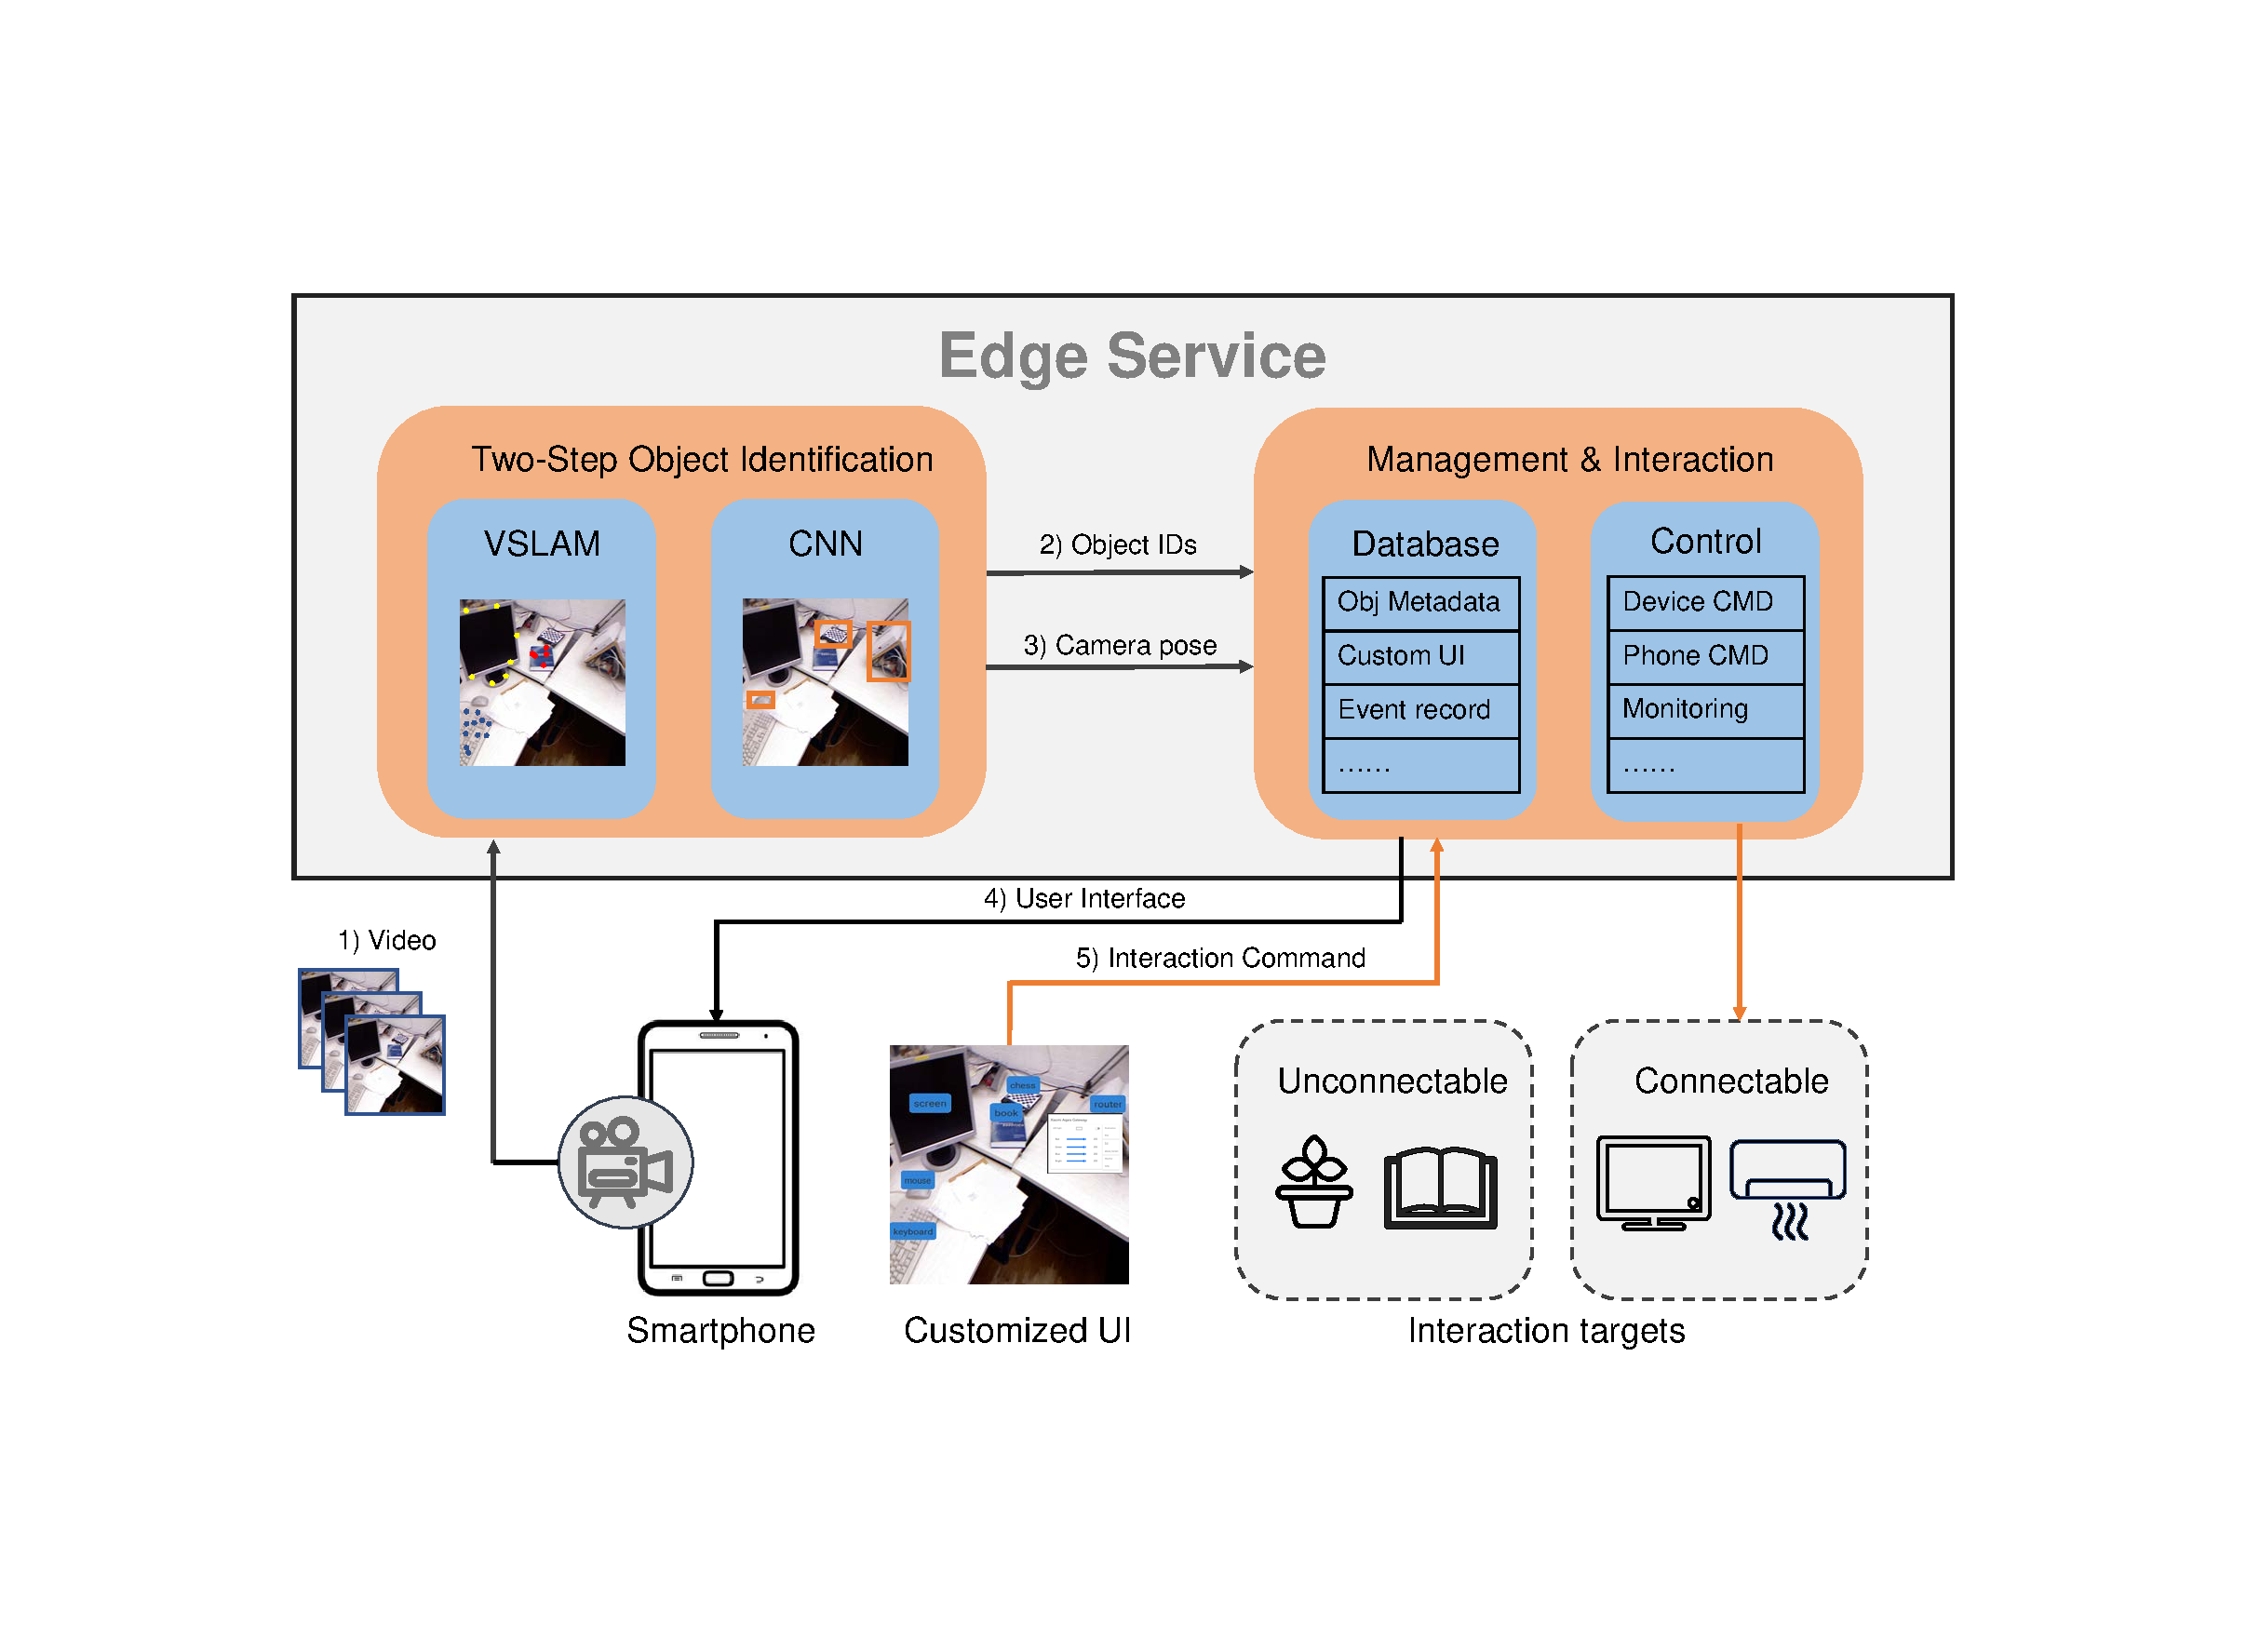
\includegraphics[width=0.99\linewidth]{overview}
	\caption{VSLink的架构:来自手机的视频帧被送往边缘服务,并将对应的UI送回手机端,用户可以使用UI进行交互}
	\label{fig:overview}
\end{figure}

\chapter{系统架构}\label{sec:architec}


图\ref{fig:overview} 显示了我们提出的VSLink的体系结构。在高层次上,交互涉及三个端,即移动设备端、边缘服务端和对象端。我们可以将交互流程总结如下。首先,用户使用智能手机对周围环境进行视频监控,视频帧通过无线链路发送到边缘服务端。第二,边缘服务识别视频帧中的对象。相应的用户界面(UI)及其位置将发送到智能手机。第三,手机在对象的位置显示UI,用户通过操作UI输入交互命令。最后,该命令由对象/手机/边缘服务根据命令属性进行处理。

为了实现上述流程并实现用户体验的准确性、速度和质量的目标,在边缘服务端我们提出了两个模块,即两阶段目标识别和对象管理与交互。目标识别模块识别当前帧中的对象,并在较低延迟内返回其ID和位置。该模块借鉴Visual SLAM和目标检测神经网络的功能,实现快速准确的目标识别。具体来说,我们提前构建了环境的对象级SLAM映射。每次启动VSLink时,边缘服务端都会执行一个Visual SLAM线程。在通过构建的地图定位Visual SLAM的过程中,我们可以使用视觉特征点描述符匹配来识别位置稳定相对背景不动的对象。此外,为了处理移动目标,采用了目标检测神经网络。将Visual SLAM识别结果作为先验,提出了一种基于稀疏卷积的方法,避免了冗余计算。一旦一个物体被神经网络检测到,我们就使用图像检索方法来识别它的ID。

对象管理与交互模块实现了实际的人机交互。如果用户命令是由对象执行的,它会将用户命令发送给对象。例如,命令是打开某个设备。为了转发命令,边缘服务端与这些可连接对象建立连接,并集成它们的API。对于不可连接的对象,VSLink也提供了实现交互的功能,这主要依赖于智能手机的功能。

\chapter{两阶段目标识别}\label{sec:fast}
\section{动机}\label{subsec:motivation}
在计算机视觉领域,识别图像/视频中感兴趣的目标已经得到了很好的研究。例如,图像分类\cite{he2019bag}、目标检测\cite{zou2019object}、图像检索\cite{philbin2008lost,zheng2017sift}和图像定位\cite{sattler2011fast}可以实现不同程度的目标识别。在表\ref{table:methods}中,我们列出了这些方法的特点,但它们都不符合第\ref{sec:introduction}章中提到的要求。因此,我们将“目标检测+图像检索”方法与Visual SLAM相结合,以实现我们的目标识别。我们之所以选择这两种方法,是因为它们在许多方面表现出互补性。我们可以把环境中的物体大致分为两类,稳定的和可移动的。稳定物体往往位于固定位置,例如电视和空调。可移动的通常从一个地方移动到另一个地方。“对象检测+图像检索”方法(为了简化表示,我们在下面省略图像检索)能够识别所有对象,但由于需要经过神经网络运算,所以速度较慢,而Visual SLAM可以识别稳定对象且速度较快。

图\ref{fig:two-step-workflow}显示了所提出的两阶段目标识别方法的框架。这种设计接近于实际人脑的工作方式。例如,如果一个人进入卧室,她/他可以立即知道电视的位置,并对自己进行基本定位。然而,要识别手机,他需要集中注意力搜索。因此从直觉上来说,我们可以利用Visual SLAM的空间感知快速识别稳定的对象,然后让神经网络处理可能发生移动的对象。同时,神经网络不需要对整个图像进行分析,只需要对SLAM未识别的区域进行分析,可以大大减少时间开销。


\begin{table}[htbp]
    \centering
    \caption{\label{table:methods}现有目标识别解决方案的可行性}
    \begin{tabular}{|l|l|l|l|l|l|l|}\hline
    方法 &
      分类 &
      ID &
      多目标 &
      移动 &
      环境改变 &
      速度 \\
      \hline 图像分类\cite{he2019bag} &
      {\color[HTML]{355421} √} &
      {\color[HTML]{BF0000} ×} &
      {\color[HTML]{BF0000} ×} &
      {\color[HTML]{355421} √} &
      {\color[HTML]{355421} √} &
      {\color[HTML]{355421} 快} \\ \hline
    目标检测\cite{zou2019object} &
      {\color[HTML]{355421} √} &
      {\color[HTML]{BF0000} ×} &
      {\color[HTML]{355421} √} &
      {\color[HTML]{355421} √} &
      {\color[HTML]{355421} √} &
      {\color[HTML]{BF0000} 慢} \\ \hline
    图像检索\cite{philbin2008lost,zheng2017sift} &
      {\color[HTML]{BF0000} ×} &
      {\color[HTML]{355421} √} &
      {\color[HTML]{BF0000} ×} &
      {\color[HTML]{355421} √} &
      {\color[HTML]{355421} √} &
      {\color[HTML]{355421} 快} \\ \hline
    检测+检索 &
      {\color[HTML]{355421} √} &
      {\color[HTML]{355421} √} &
      {\color[HTML]{355421} √} &
      {\color[HTML]{355421} √} &
      {\color[HTML]{355421} √} &
      {\color[HTML]{BF0000} 慢} \\ \hline
    图像定位\cite{sattler2011fast} &
      {\color[HTML]{BF0000} ×} &
      {\color[HTML]{355421} √} &
      {\color[HTML]{355421} √} &
      {\color[HTML]{BF0000} ×} &
      {\color[HTML]{BF0000} ×} &
      {\color[HTML]{BF0000} 慢} \\ \hline
    Visual SLAM\cite{liu2021edgesharing} &
      {\color[HTML]{BF0000} ×} &
      {\color[HTML]{355421} √} &
      {\color[HTML]{355421} √} &
      {\color[HTML]{BF0000} ×} &
      {\color[HTML]{BF0000} ×} &
      {\color[HTML]{355421} 快} \\ \hline
    \end{tabular}
    \end{table}

    \begin{figure}[t]
        \centering
        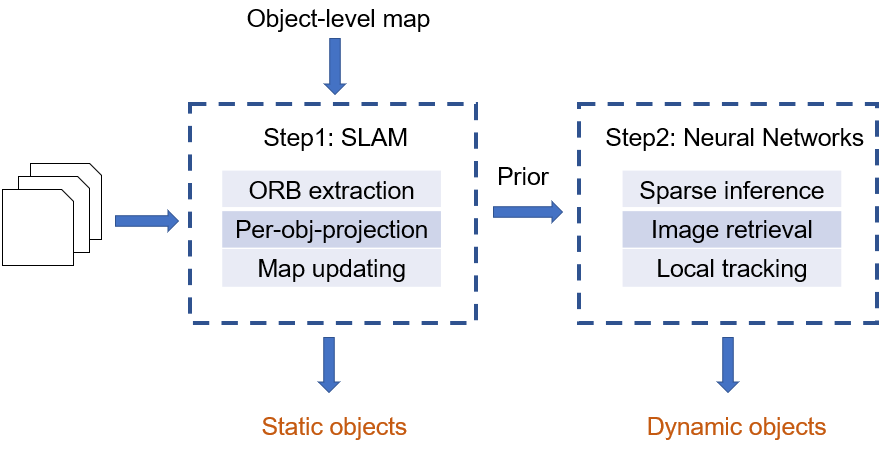
\includegraphics[width=0.75\linewidth]{twostep}
        \caption{两阶段目标识别方法框架}
        \label{fig:two-step-workflow}
    \end{figure}

    \begin{figure}[t]
        \centering
        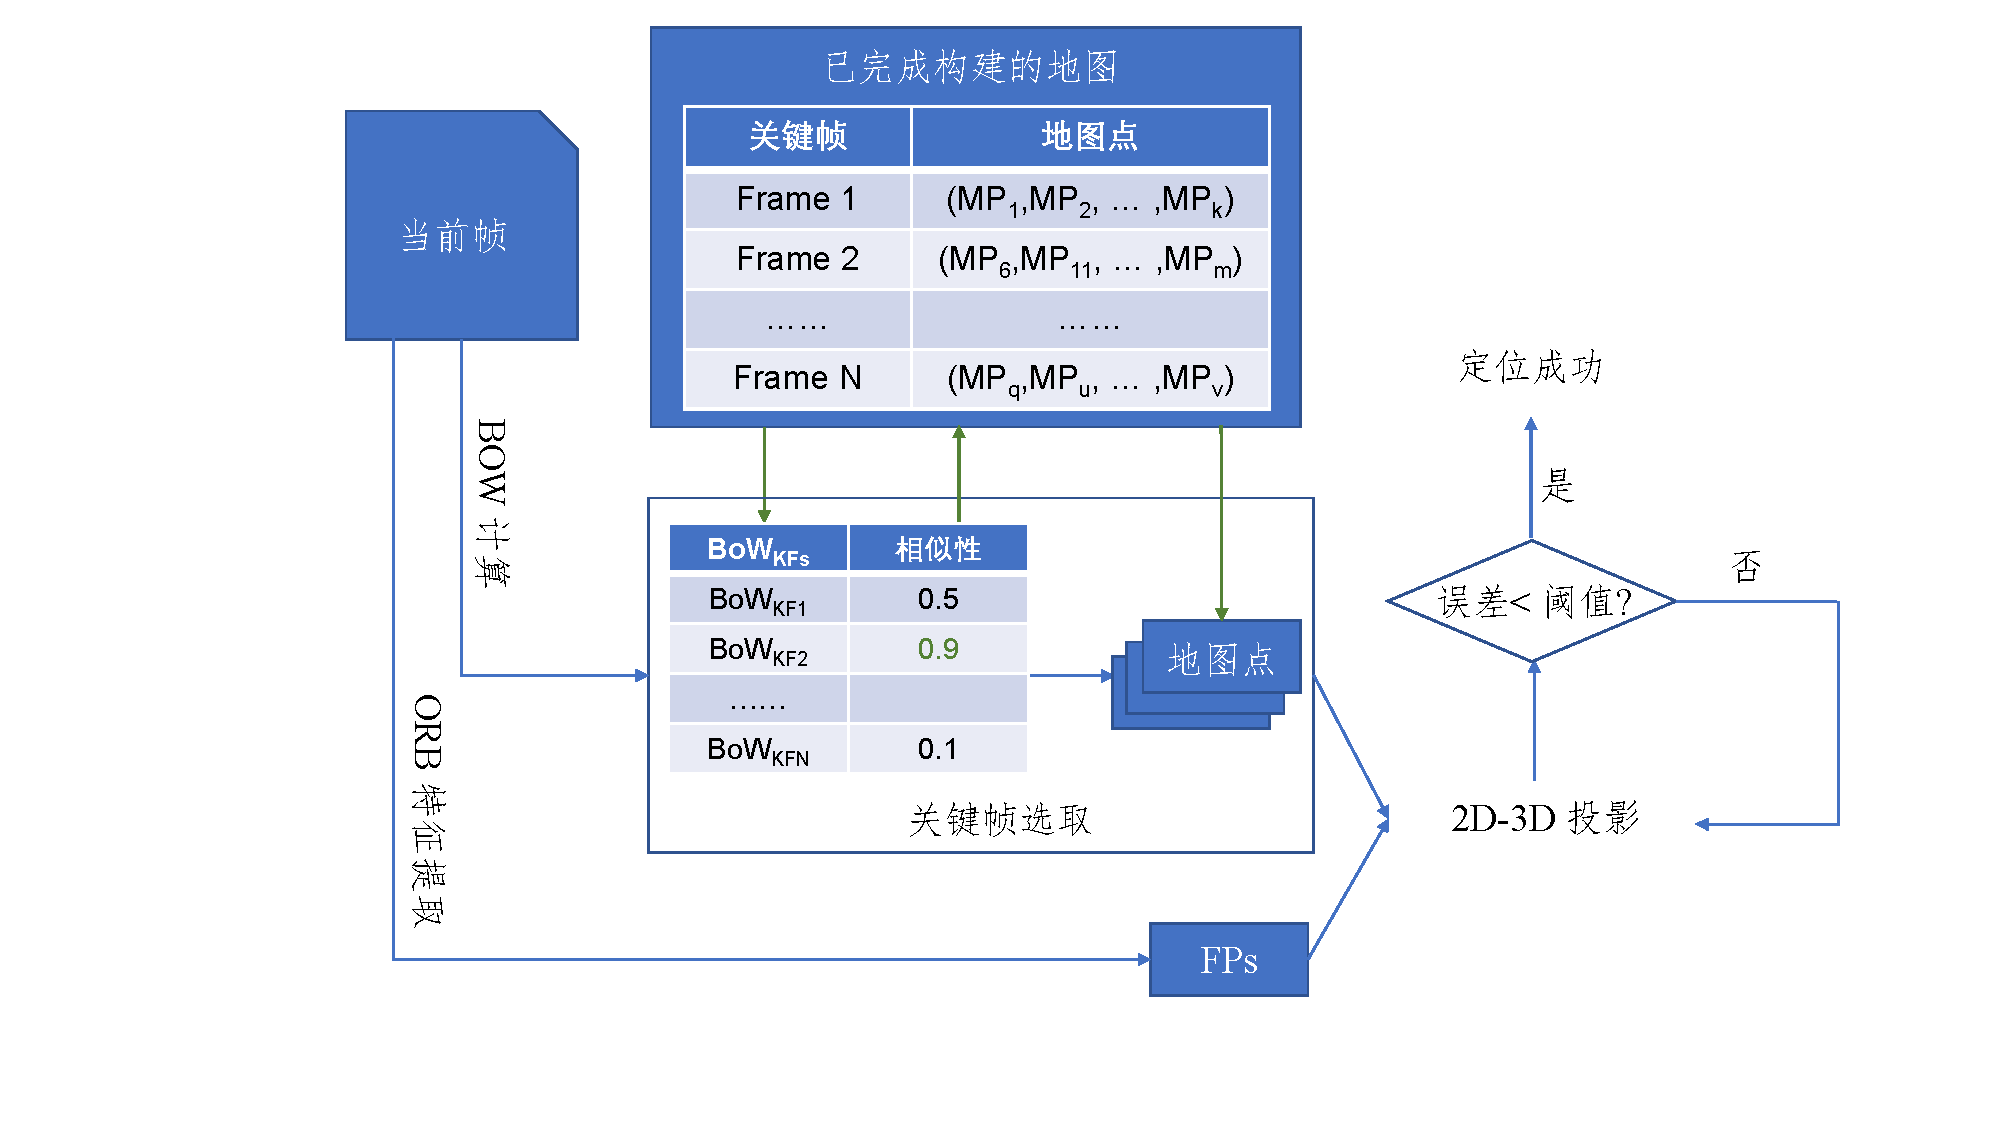
\includegraphics[width=0.8\linewidth]{workflow}
        \caption{Localization process of ORB-SLAM~\cite{mur2017orb} during map reuse.}
        \label{fig:localization}
    \end{figure}
\section{基于Visual SLAM的目标识别}
SLAM被认为是实现更真实AR体验的关键技术之一,因为它提供了对环境的理解和跟踪。在VSLink中,我们建议建立一个终身对象级SLAM映射,这有利于SLAM跟踪和对象识别。

1) 工作流:在这里,我们解释了所提出的基于Visual SLAM的对象识别解决方案的理论。由于经典的VS-LAM[18],[19]技术试图在机器人第一次进入环境时实现精确的映射和定位,我们想知道机器人第二次进入环境时是否能够识别它所看到的物体。

构建的SLAM地图[18]仅包括某些地图点和关键帧,地图重用过程如图3所示。定位过程首先使用单词包(BoW)[20]计算当前帧的表示,然后计算当前帧和关键帧之间的BoW相似性。然后,它选择具有高弓相似性的关键帧作为候选帧。最后,对于每个选定的关键帧,它使用RANSAC[21]算法计算当前帧中的特征点与该关键帧的贴图点之间的2D-3D投影。如果投影误差小于阈值,则定位完成。


\chapter{参考命令}
\section{节标题}

我们可以用includegraphics来插入现有的jpg等格式的图片,
如\autoref{fig:zju-logo}所示。

\begin{figure}[htbp]
    \centering
    \includegraphics[width=.3\linewidth]{logo/zju}
    \caption{\label{fig:zju-logo}浙江大学LOGO}
\end{figure}


\subsection{小节标题}


\par 如\autoref{tab:sample}所示,这是一张自动调节列宽的表格。

\begin{table}[htbp]
    \caption{\label{tab:sample}自动调节列宽的表格}
    \begin{tabularx}{\linewidth}{c|X<{\centering}}
        \hline
        第一列 & 第二列 \\ \hline
        xxx & xxx \\ \hline
        xxx & xxx \\ \hline
        xxx & xxx \\ \hline
    \end{tabularx}
\end{table}


\par 如\autoref{equ:sample},这是一个公式

\begin{equation}
    \label{equ:sample}
    A=\overbrace{(a+b+c)+\underbrace{i(d+e+f)}_{\text{虚数}}}^{\text{复数}}
\end{equation}

\chapter{另一章}


\begin{figure}[htbp]
    \centering
    \includegraphics[width=.3\linewidth]{example-image-a}
    \caption{\label{fig:fig-placeholder}图片占位符}
\end{figure}